\documentclass[tikz]{standalone}
\usepackage{pgfplots}
\pgfplotsset{compat=newest}
\pgfplotsset{every axis legend/.append style={%
cells={anchor=west}}
}
\usetikzlibrary{arrows}
\tikzset{>=stealth'}

\begin{document}
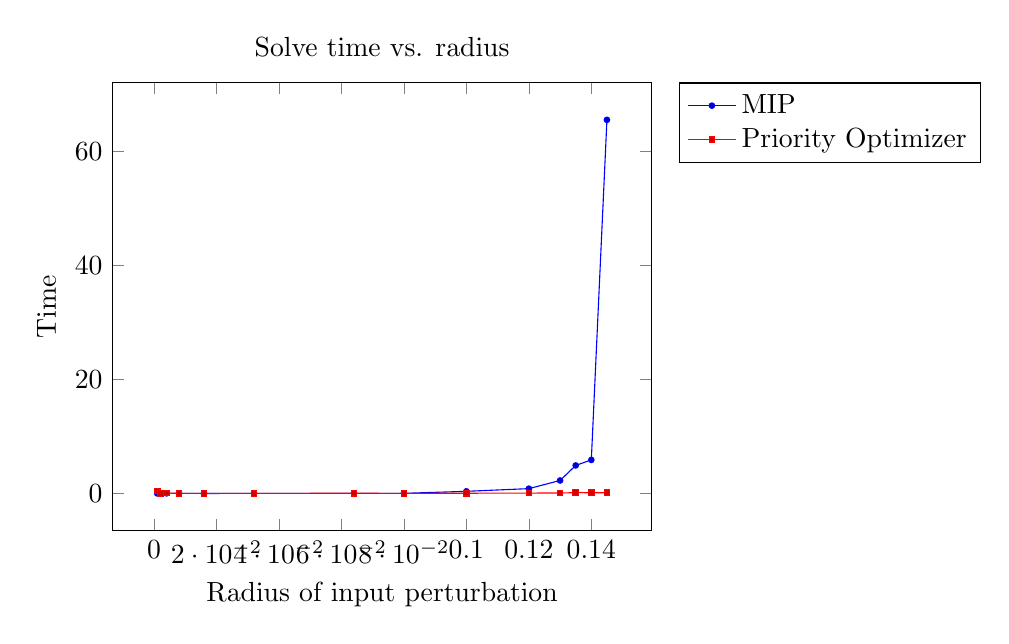
\begin{tikzpicture}[]
\begin{axis}[
  legend style = {at={(1.05,1.0)}, anchor = north west},
  ylabel = {Time},
  title = {Solve time vs. radius},
  xlabel = {Radius of input perturbation},
  black
]

\addplot+[
  mark size = {1.0}
] coordinates {
  (0.001, 0.019233845)
  (0.002, 0.022304629)
  (0.004, 0.031418115)
  (0.008, 0.030623215)
  (0.016, 0.014900793)
  (0.032, 0.022915338)
  (0.064, 0.034330358)
  (0.08, 0.037327517)
  (0.1, 0.389828453)
  (0.12, 0.860928497)
  (0.13, 2.293617902)
  (0.135, 4.928446751)
  (0.14, 5.899929212)
  (0.145, 65.541657653)
};
\addlegendentry{{}{MIP}}

\addplot+[
  mark size = {1.0}
] coordinates {
  (0.001, 0.465945696)
  (0.002, 0.018623026)
  (0.004, 0.071476041)
  (0.008, 0.036081881)
  (0.016, 0.042230627)
  (0.032, 0.025753228)
  (0.064, 0.055634719)
  (0.08, 0.029579747)
  (0.1, 0.056198651)
  (0.12, 0.084520705)
  (0.13, 0.091574042)
  (0.135, 0.161171113)
  (0.14, 0.139801583)
  (0.145, 0.140682861)
};
\addlegendentry{{}{Priority Optimizer}}

\end{axis}
\end{tikzpicture}

\end{document}
